\chapter{QCD NNLO/NLO k-factors for qq $\rightarrow$ ZZ}
\label{app:kfactor_qcd_zz}

The NNLO/NLO $K$-factors for the qq$\rightarrow$ZZ process are available binned in different generator-level variables.
They can be applied as a function of either the the transverse momentum $p_{T}(Z,Z)$,
invariant mass $M(Z,Z)$ or angular separation $\Delta\phi(Z,Z)$ of the diboson system.
While all three versions of the $K$-factors stem from the same calculation framework and are thus in agreement as far
as calculation settings are observed, the binning may impact the result of the corrections.
The $K$-factors are shown in fig.~\ref{fig:kfactor_qcd_zz}, the distributions of the generator-level variables are shown in fig.~\ref{fig:genvars_qcd_zz}.
The generator variables are shown for simulated ZZ events after applying the final analysis selection.
For both $\Delta\phi(Z,Z)$ and $p_{T}(Z,Z)$, the signal region events are very strongly peaked in regions where the $K$-factors are significantly non-flat.
The application of these $K$-factors thus strongly depends on the choice of bin sizes. Small variation of the bin sizes may induce large changes in the medium
k-factor per bin. To avoid the complications associated with this, the $M(Z,Z)$-binning is used. In this case, the signal region events are not contained in a
region of large $K$-factors variations and the correction is thus more reliable.

\begin{figure}[htbp]
\begin{center}
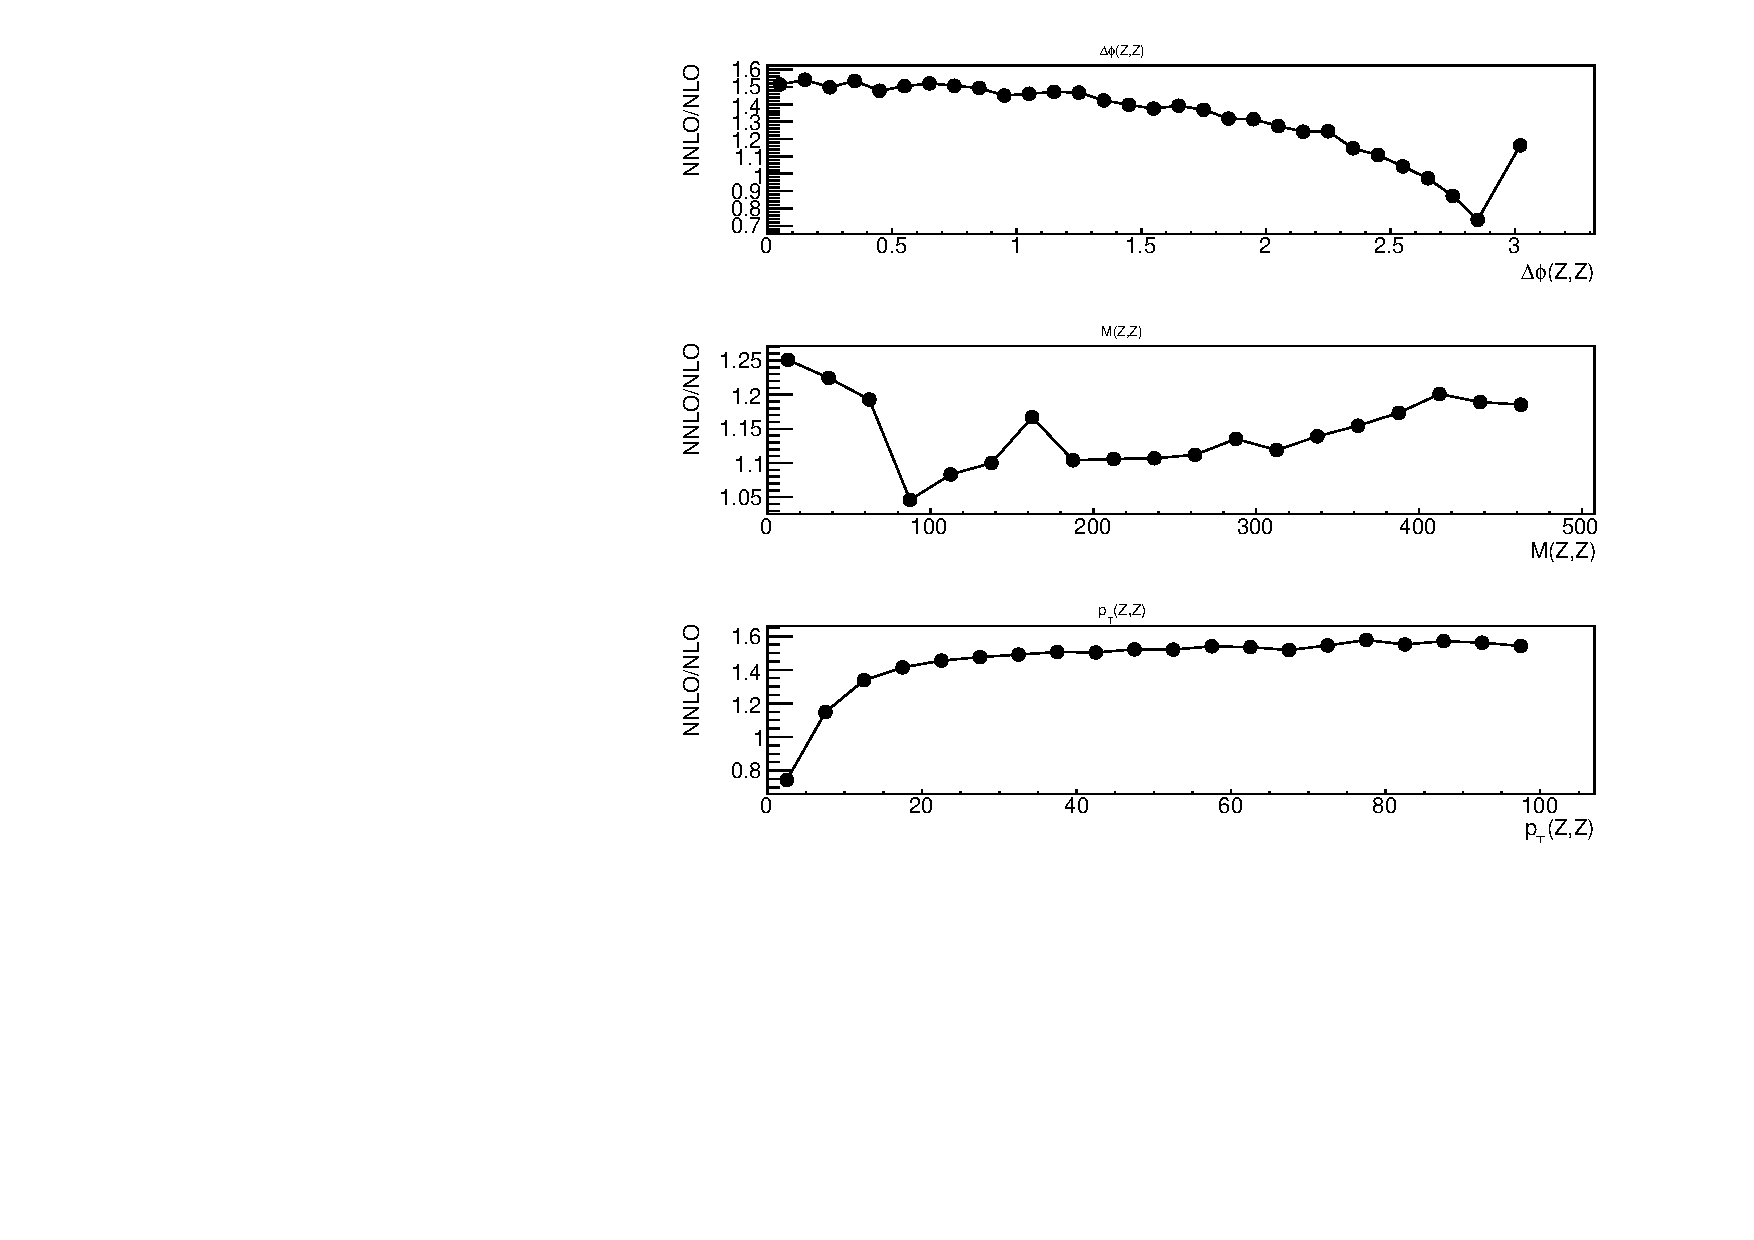
\includegraphics[width=\textwidth]{figures/kfactors.pdf}
\caption{QCD NNLO/NLO k factors for the qq$\rightarrow$ZZ process binned in different generator-level kinematic variables of the diboson system.
}
\label{fig:kfactor_qcd_zz}
\end{center}
\end{figure}

\begin{figure}[htbp]
\begin{center}
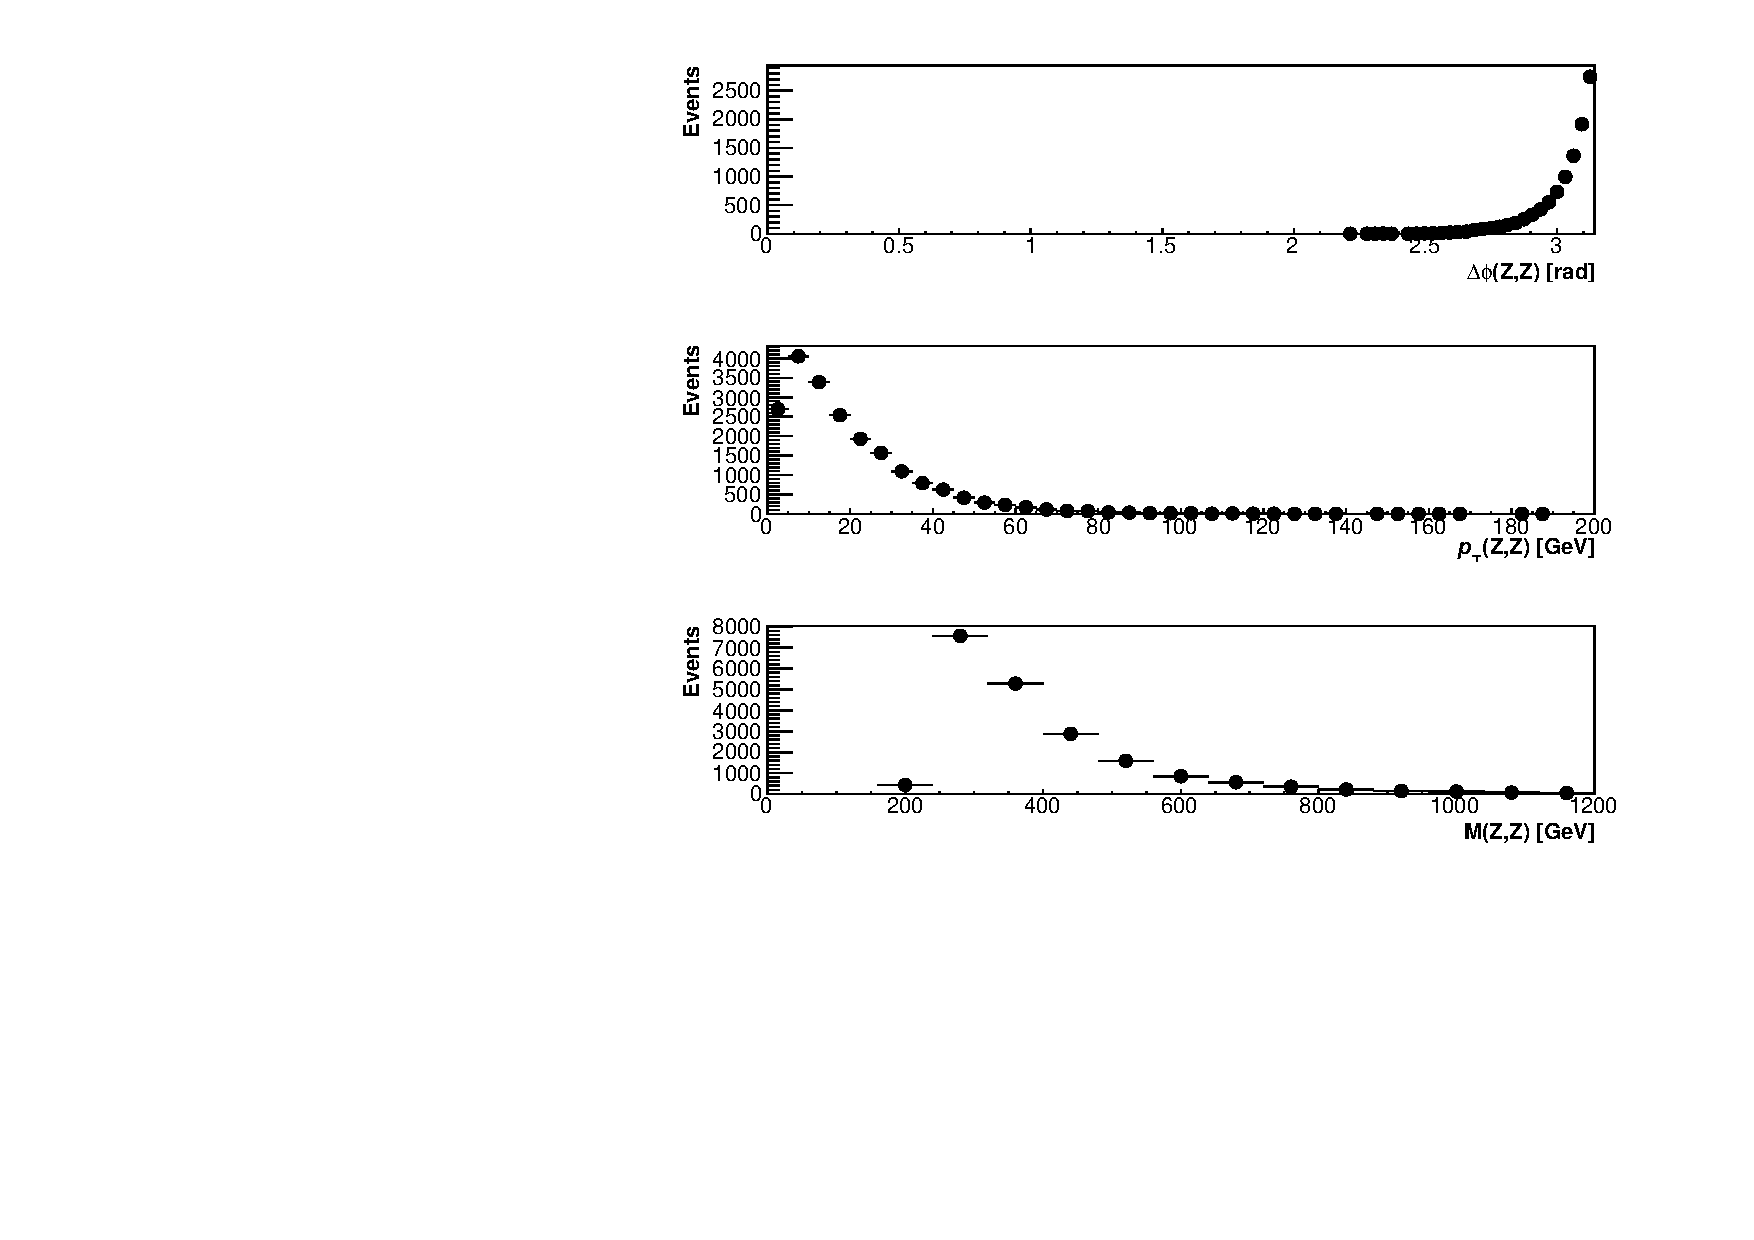
\includegraphics[width=\textwidth]{figures/genvars.pdf}
\caption{Distribution of the generator-level kinematic variables of the diboson system in ZZ events after final selection.
}
\label{fig:genvars_qcd_zz}
\end{center}
\end{figure}

